\chapter{Foundations: What Is Mathematics?}\index{foundations}\index{mathematics!nature of}

\section{The Building Blocks of Thought}

\begin{intuition}
Before we can do mathematics, we must answer a fundamental question: \textit{What is mathematics?} 

Is it the study of numbers? Shapes? Patterns? While mathematics involves all of these, its true nature is more abstract. Mathematics is the art of \textbf{reasoning with perfect precision} about abstract objects.

This chapter starts informally. We'll use everyday language to explain what we're building toward. Think of this as the \textit{construction site} before the building exists.
\end{intuition}

\subsection{A Simple Example: Counting}

Let's start with something familiar: counting. When you count objects---say, apples---you say ``1, 2, 3, 4, 5.'' This seems natural. But what are you \textit{actually} doing?

\begin{enumerate}
    \item You're matching each apple to a word: ``one,'' ``two,'' ``three,'' etc.
    \item You're following rules: don't skip numbers, don't count the same apple twice
    \item You're using symbols: the marks ``1'', ``2'', ``3'' represent abstract concepts
\end{enumerate}

Here's the key insight: \textbf{the numbers themselves don't exist in physical reality}. You can't touch ``five.'' You can touch five apples, but ``five-ness'' itself is abstract. Mathematics studies these abstractions.

\vspace{0.5cm}
\begin{center}
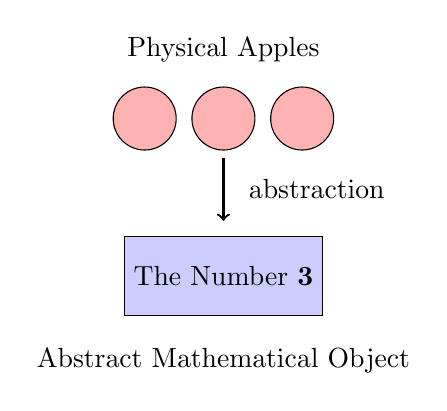
\begin{tikzpicture}
    % Physical apples
    \node[circle, draw, fill=red!30, minimum size=0.8cm] at (0,2) {};
    \node[circle, draw, fill=red!30, minimum size=0.8cm] at (1,2) {};
    \node[circle, draw, fill=red!30, minimum size=0.8cm] at (2,2) {};
    \node[above] at (1,2.6) {Physical Apples};
    
    % Arrow
    \draw[->, thick] (1,1.5) -- (1,0.7);
    \node[right] at (1.2,1.1) {abstraction};
    
    % Abstract number
    \node[rectangle, draw, fill=blue!20, minimum width=2cm, minimum height=1cm] at (1,0) {The Number \textbf{3}};
    \node[below] at (1,-0.8) {Abstract Mathematical Object};
\end{tikzpicture}
\end{center}
\vspace{0.5cm}

\subsection{The Need for Precision}

In everyday life, we can be vague. If I say ``Meet me around 3 PM,'' you understand I might arrive at 2:58 or 3:05. But in mathematics, we can't be vague.

\begin{example}[Vague vs. Precise]
\textbf{Vague statement:} ``Large numbers grow quickly.''

\textbf{Questions this raises:}
\begin{itemize}
    \item What counts as ``large''? 100? 1,000,000?
    \item What does ``quickly'' mean? Compared to what?
    \item What does ``grow'' mean? As we add? Multiply?
\end{itemize}

\textbf{Precise statement:} ``For any real number $M > 0$, there exists a natural number $N$ such that $2^n > M$ for all $n > N$.''

Now there's no ambiguity. Every word has exact meaning.
\end{example}

\begin{keyidea}
Mathematics requires a language with \textbf{zero ambiguity}. Every statement must have exactly one interpretation. This is why we need formal systems.
\end{keyidea}

\section{The Game of Mathematics}

\subsection{Mathematics as a Game}

Think of mathematics as a sophisticated game, like chess:

\vspace{0.5cm}
\begin{center}
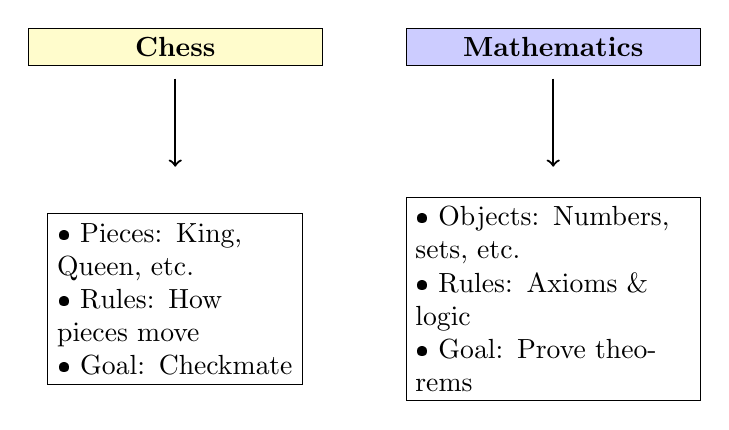
\begin{tikzpicture}[scale=0.8]
    % Chess analogy
    \node[rectangle, draw, fill=yellow!20, text width=3.5cm, align=center] at (0,4) {\textbf{Chess}};
    \node[rectangle, draw, fill=blue!20, text width=3.5cm, align=center] at (6,4) {\textbf{Mathematics}};
    
    \draw[->, thick] (0,3.5) -- (0,2.1);
    \draw[->, thick] (6,3.5) -- (6,2.1);
    
    \node[rectangle, draw, text width=3cm, align=left] at (0,0) {
        • Pieces: King, Queen, etc.\\
        • Rules: How pieces move\\
        • Goal: Checkmate
    };
    
    \node[rectangle, draw, text width=3.5cm, align=left] at (6,0) {
        • Objects: Numbers, sets, etc.\\
        • Rules: Axioms \& logic\\
        • Goal: Prove theorems
    };
\end{tikzpicture}
\end{center}
\vspace{0.5cm}

\textbf{In chess:}
\begin{itemize}
    \item \textbf{Pieces} are the objects you manipulate
    \item \textbf{Rules} say what moves are legal
    \item \textbf{Strategy} is how you win, but it's not part of the rules
\end{itemize}

\textbf{In mathematics:}
\begin{itemize}
    \item \textbf{Mathematical objects} are what we study (numbers, shapes, functions, etc.)
    \item \textbf{Axioms and logic} are the rules
    \item \textbf{Theorems} are the ``wins''---statements we prove are true
\end{itemize}

\subsection{What Are Symbols?}

When you see ``$2 + 3 = 5$'', what is it? It's a string of symbols:
\begin{center}
$2$ \quad $+$ \quad $3$ \quad $=$ \quad $5$
\end{center}

Each symbol is just a mark on paper (or pixels on a screen). The symbols themselves have no inherent meaning. We \textit{give them meaning} by agreeing on what they represent.

\vspace{0.5cm}
\begin{center}
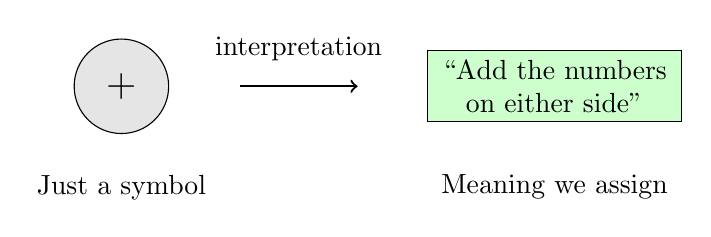
\begin{tikzpicture}
    \node[circle, draw, fill=gray!20, minimum size=1.2cm] at (0,0) {\Large $+$};
    \node[below] at (0,-1) {Just a symbol};
    
    \draw[->, thick] (1.5,0) -- (3,0);
    \node[above] at (2.25,0.2) {interpretation};
    
    \node[rectangle, draw, fill=green!20, text width=3cm, align=center] at (5.5,0) {``Add the numbers\\on either side''};
    \node[below] at (5.5,-1) {Meaning we assign};
\end{tikzpicture}
\end{center}
\vspace{0.5cm}

\begin{warning}
Symbols are NOT the same as their meanings. The symbol ``$+$'' is different from the concept of addition. We could have used any symbol---say ``$\oplus$'' or ``\&''---as long as we agreed on the meaning.

This distinction between \textbf{syntax} (symbols) and \textbf{semantics} (meaning) is crucial for understanding formal mathematics.
\end{warning}

\section{Building Mathematics from Scratch}

\subsection{The Bootstrap Problem}

We face a philosophical problem: to explain mathematics, we're using language (English). But language itself is imprecise. We're trying to build something precise using imprecise tools!

This is like trying to build a perfectly straight ruler when you don't have any straight edge to measure against.

\vspace{0.5cm}
\begin{center}
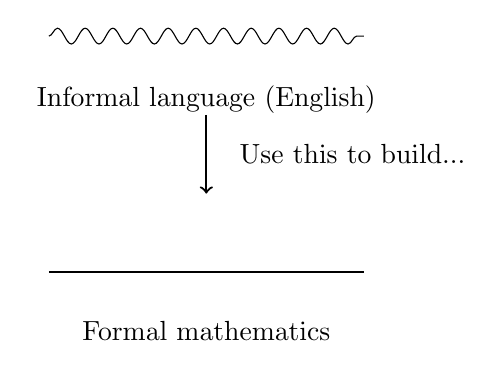
\begin{tikzpicture}
    \draw[decorate, decoration={snake, amplitude=1mm}] (0,0) -- (4,0);
    \node[below] at (2,-0.5) {Informal language (English)};
    
    \draw[->, thick] (2,-1) -- (2,-2);
    \node[right] at (2.3,-1.5) {Use this to build...};
    
    \draw[thick] (0,-3) -- (4,-3);
    \node[below] at (2,-3.5) {Formal mathematics};
\end{tikzpicture}
\end{center}
\vspace{0.5cm}

The solution is to be \textit{as clear as possible} in our informal explanations, and then formalize carefully. We'll use everyday language to explain concepts, but we'll mark the transition when we go formal.

\subsection{The Ladder of Abstraction}

Mathematics is built in layers. Each layer assumes the one below it:

\vspace{0.5cm}
\begin{center}
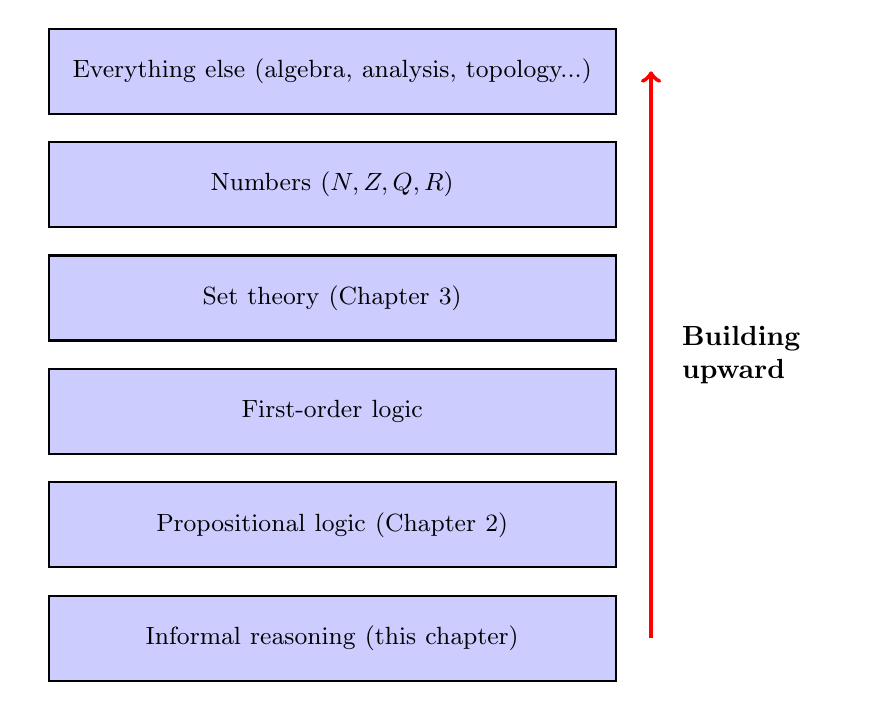
\begin{tikzpicture}[scale=0.9]
    % Draw the ladder
    \foreach \y/\label in {0/{Informal reasoning (this chapter)}, 
                           1.6/{Propositional logic (Chapter 2)},
                           3.2/{First-order logic},
                           4.8/{Set theory (Chapter 3)},
                           6.4/{Numbers ($\mathbb{N}, \mathbb{Z}, \mathbb{Q}, \mathbb{R}$)},
                           8/{Everything else (algebra, analysis, topology...)}} {
        \draw[thick, fill=blue!20] (-4,\y) rectangle (4,\y+1.2);
        \node[text width=7.5cm, align=center] at (0,\y+0.6) {\small \label};
    }
    
    % Arrow showing direction of building
    \draw[->, ultra thick, red] (4.5,0.6) -- (4.5,8.6);
    \node[right, text width=2cm] at (4.8,4.6) {\textbf{Building upward}};
\end{tikzpicture}
\end{center}
\vspace{0.5cm}

\begin{intuition}
You can't understand calculus without algebra. You can't understand algebra without numbers. You can't understand numbers without set theory. You can't understand set theory without logic. 

This book starts at the bottom and works up. Be patient. The early chapters might seem overly detailed, but they're the foundation for everything that follows.
\end{intuition}

\section{Strings and Expressions}

Let's start building. The most basic concept is a \textbf{string of symbols}.

\subsection{Alphabets}

\begin{definition}[Alphabet---Informal]
An \textbf{alphabet} is a collection of symbols. These are our basic building blocks.
\end{definition}

\begin{example}[Familiar Alphabets]
\begin{enumerate}
    \item \textbf{English alphabet}: $\{a, b, c, \ldots, z, A, B, C, \ldots, Z\}$
    \item \textbf{Decimal digits}: $\{0, 1, 2, 3, 4, 5, 6, 7, 8, 9\}$
    \item \textbf{Binary}: $\{0, 1\}$
    \item \textbf{Mathematical symbols}: $\{+, -, \times, \div, =, (, ), x, y, \ldots\}$
\end{enumerate}
\end{example}

Think of an alphabet as your box of Scrabble tiles. You have a fixed set of letters (symbols) to work with.

\subsection{Strings}

\begin{definition}[String---Informal]
A \textbf{string} (or \textbf{expression}) is a sequence of symbols from an alphabet, written one after another.
\end{definition}

\begin{example}[Strings]
Using the English alphabet:
\begin{itemize}
    \item \texttt{cat} is a string of length 3
    \item \texttt{hello} is a string of length 5  
    \item \texttt{xyz} is a string of length 3
    \item \texttt{aaa} is a string of length 3 (repetition is allowed)
    \item The empty string (no symbols) is also a string, written $\varepsilon$
\end{itemize}
\end{example}

\vspace{0.5cm}
\begin{center}
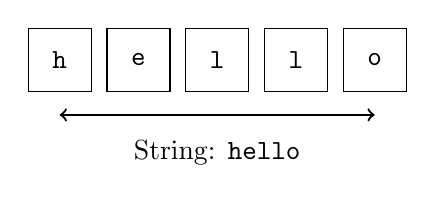
\begin{tikzpicture}
    % Show string as sequence
    \foreach \x/\letter in {0/h, 1/e, 2/l, 3/l, 4/o} {
        \node[rectangle, draw, minimum size=0.8cm] at (\x,0) {\texttt{\letter}};
    }
    \draw[<->, thick] (0,-0.7) -- (4,-0.7);
    \node[below] at (2,-0.9) {String: \texttt{hello}};
\end{tikzpicture}
\end{center}
\vspace{0.5cm}

\textbf{Key point:} A string is just symbols in order. It doesn't have to "mean" anything. The string \texttt{xqzp} is perfectly valid, even though it's not an English word.

\subsection{Concatenation}

\begin{definition}[Concatenation---Informal]
\textbf{Concatenation} means sticking two strings together, end-to-end.
\end{definition}

\begin{example}
\begin{itemize}
    \item \texttt{cat} concatenated with \texttt{dog} gives \texttt{catdog}
    \item \texttt{hello} concatenated with \texttt{world} gives \texttt{helloworld}
    \item \texttt{123} concatenated with \texttt{456} gives \texttt{123456} (note: this is NOT addition!)
\end{itemize}
\end{example}

\vspace{0.5cm}
\begin{center}
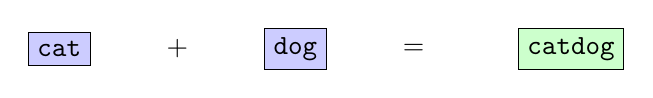
\begin{tikzpicture}
    \node[rectangle, draw, fill=blue!20] at (0,0) {\texttt{cat}};
    \node at (1.5,0) {$+$};
    \node[rectangle, draw, fill=blue!20] at (3,0) {\texttt{dog}};
    \node at (4.5,0) {$=$};
    \node[rectangle, draw, fill=green!20] at (6.5,0) {\texttt{catdog}};
\end{tikzpicture}
\end{center}
\vspace{0.5cm}

\begin{remark}
Concatenation has some nice properties:
\begin{itemize}
    \item \textbf{Associative}: $(s \cdot t) \cdot u = s \cdot (t \cdot u)$
    \item \textbf{Identity}: Concatenating with the empty string does nothing: $s \cdot \varepsilon = \varepsilon \cdot s = s$
    \item \textbf{NOT commutative}: Generally $s \cdot t \neq t \cdot s$ (e.g., \texttt{catdog} $\neq$ \texttt{dogcat})
\end{itemize}
\end{remark}

\section{Meaning vs. Form}

\subsection{Syntax and Semantics}

Now we reach a crucial distinction that underpins all of formal mathematics:

\begin{definition}[Syntax---Informal]
\textbf{Syntax} is the study of form---what strings of symbols look like, how they're constructed, which ones are "well-formed."
\end{definition}

\begin{definition}[Semantics---Informal]
\textbf{Semantics} is the study of meaning---what strings of symbols represent, what they "say."
\end{definition}

\begin{example}[Syntax vs. Semantics]
Consider the expression: $2 + 3$

\textbf{Syntactically:} This is a string of 5 symbols: ``$2$'', ``$ $'', ``$+$'', ``$ $'', ``$3$''
(Yes, the spaces are symbols too!)

\textbf{Semantically:} Under the usual interpretation, this represents the sum of two and three, which equals five.

But we could define a different interpretation where ``$+$'' means multiplication. Then $2 + 3$ would mean $2 \times 3 = 6$.
\end{example}

\vspace{0.5cm}
\begin{center}
\begin{tikzpicture}[node distance=2cm]
    % Top: Expression
    \node[rectangle, draw, fill=yellow!20, minimum width=3cm, minimum height=1cm] (expr) {$2 + 3$};
    
    % Left branch: Syntax
    \node[rectangle, draw, fill=blue!20, text width=3cm, align=center, below left=2.5cm and 1.5cm of expr] (syntax) {\textbf{Syntax}\\String of 3 symbols};
    
    % Right branch: Semantics
    \node[rectangle, draw, fill=green!20, text width=3cm, align=center, below right=of expr] (semantics) {\textbf{Semantics}\\The number 5};
    
    \draw[->, thick] (expr) -- (syntax);
    \draw[->, thick] (expr) -- (semantics);
    
    \node[below=0.3cm of syntax, text width=3cm, align=center] {\small Form/Structure};
    \node[below=0.3cm of semantics, text width=3cm, align=center] {\small Meaning/Interpretation};
\end{tikzpicture}
\end{center}
\vspace{0.5cm}

\begin{keyidea}
In formal mathematics:
\begin{enumerate}
    \item First, we define syntax: which strings are valid
    \item Then, we define semantics: what those strings mean
\end{enumerate}

This separation is crucial. We can manipulate symbols without knowing what they mean (syntax), and then interpret the results (semantics).
\end{keyidea}

\subsection{Why Separate Syntax and Semantics?}

You might wonder: why bother separating form from meaning? Can't we just work with meaningful statements?

The answer is: separating them gives us \textbf{mechanical rules}. A computer can check syntax without understanding meaning.

\begin{example}[Spell Check]
A spell checker operates purely syntactically:
\begin{itemize}
    \item It checks if words are in its dictionary (valid strings)
    \item It doesn't understand what the words mean
\end{itemize}

The sentence "Colorless green ideas sleep furiously" is syntactically correct English (adjective-adjective-noun-verb-adverb) but semantically nonsense.
\end{example}

\section{The Axiomatic Method}

\subsection{What Is an Axiom?}

We've been building up to this. Here's the central idea of modern mathematics:

\begin{definition}[Axiom---Informal]
An \textbf{axiom} is a statement we accept as true without proof. Axioms are the starting point for all reasoning in a mathematical system.
\end{definition}

\begin{intuition}
Think of axioms as the "rules of the game." In chess, you don't prove that the bishop moves diagonally---it's a rule you accept. In mathematics, we accept certain basic statements (axioms) and derive everything else from them.
\end{intuition}

\begin{example}[Euclidean Geometry Axioms]
Euclid based all of geometry on five axioms (postulates). Here's one:

\textbf{Axiom:} Through any two points, there exists exactly one straight line.

We don't prove this. We \textit{assume} it. Then we use it to prove other statements (theorems) like the Pythagorean theorem.
\end{example}

\subsection{The Axiomatic Method: How It Works}

Here's the structure of an axiomatic system:

\vspace{0.5cm}
\begin{center}
\begin{tikzpicture}[node distance=1.5cm]
    % Level 1: Axioms
    \node[rectangle, draw, fill=red!20, minimum width=3cm, minimum height=0.8cm] (ax) {\textbf{Axioms}};
    \node[left=0.3cm of ax, text width=2.5cm, align=right] {\small Assumed without proof};
    
    % Level 2: Theorems
    \node[rectangle, draw, fill=green!20, minimum width=3cm, minimum height=0.8cm, below=1.5cm of ax] (thm) {\textbf{Theorems}};
    \node[left=0.3cm of thm, text width=2.5cm, align=right] {\small Proved from axioms};
    
    % Level 3: More theorems
    \node[rectangle, draw, fill=green!20, minimum width=3cm, minimum height=0.8cm, below=1.5cm of thm] (thm2) {\textbf{More Theorems}};
    \node[left=0.3cm of thm2, text width=2.8cm, align=right] {\small Proved from earlier theorems};
    
    % Now draw arrows after all boxes are defined
    \draw[->, ultra thick] (ax.south) -- (thm.north) node[midway, right=0.3cm] {\small apply logic};
    \draw[->, ultra thick] (thm.south) -- (thm2.north) node[midway, right=0.3cm] {\small apply logic};
    
    % Continue arrow
    \draw[->, ultra thick, dashed] (thm2.south) -- ++(0,-1);
    \node[below=1.3cm of thm2] {$\vdots$};
\end{tikzpicture}
\end{center}
\vspace{0.5cm}

\textbf{The process:}
\begin{enumerate}
    \item Start with axioms (statements assumed true)
    \item Use logical rules to derive new statements (theorems)
    \item Use proved theorems to derive more theorems
    \item Continue building the mathematical structure
\end{enumerate}

\subsection{Why Axioms?}

You might ask: why not just prove everything? Why have statements we don't prove?

The answer: \textbf{we have to start somewhere}. If we had to prove every statement using earlier statements, we'd have infinite regress:

\begin{center}
To prove A, we need B. \\
To prove B, we need C. \\
To prove C, we need D. \\
$\vdots$ \\
(Never ends!)
\end{center}

Axioms break this cycle. They're our starting point.

\begin{keyidea}
An axiomatic system is like a building:
\begin{itemize}
    \item \textbf{Axioms} are the foundation
    \item \textbf{Definitions} introduce new concepts
    \item \textbf{Theorems} are the floors we build on top
    \item \textbf{Proofs} are the construction that connects them
\end{itemize}

If the foundation is solid, the building stands. If the axioms are consistent, mathematics works.
\end{keyidea}

\section{Consistency and Truth}

\subsection{Can Axioms Be Wrong?}

Here's a deep question: how do we know our axioms are "correct"?

The answer might surprise you: \textbf{we don't care if they're "true"}. We only care if they're \textbf{consistent}.

\begin{definition}[Consistency---Informal]
A set of axioms is \textbf{consistent} if you can never derive a contradiction from them---that is, you can never prove both a statement and its negation.
\end{definition}

\begin{example}[Inconsistent Axioms]
Suppose we had these axioms:
\begin{enumerate}
    \item All numbers are positive
    \item $-5$ is a number
\end{enumerate}

These are inconsistent! From (1) and (2), we can derive that $-5$ is positive. But $-5$ is also negative (by definition). Contradiction!

Such a system is useless because we can prove anything (including false statements).
\end{example}

\begin{example}[Different Consistent Systems]
Consider these two axiom systems:

\textbf{System A:} Euclid's five postulates (including the parallel postulate)
$\to$ Gives Euclidean geometry (flat space)

\textbf{System B:} Euclid's first four postulates + negation of the parallel postulate
$\to$ Gives hyperbolic geometry (curved space)

Both are consistent! They just describe different mathematical universes. Neither is "wrong"---they're just different.
\end{example}

\vspace{0.5cm}
\begin{center}
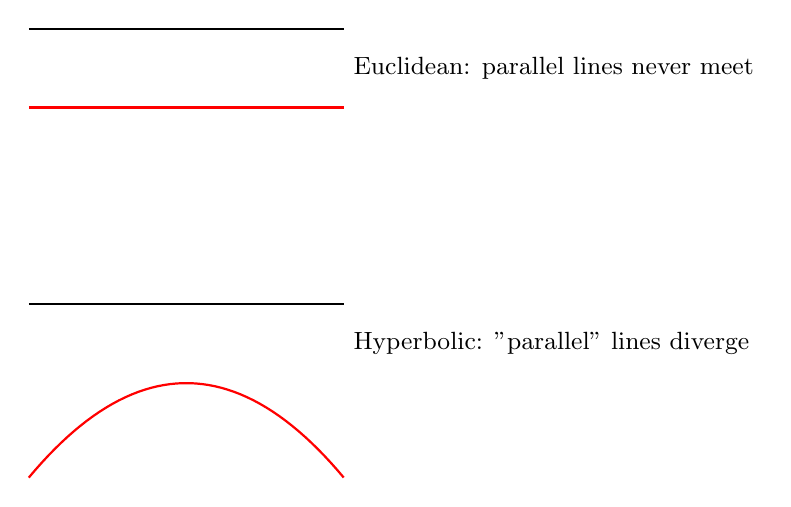
\begin{tikzpicture}
    % Euclidean
    \draw[thick] (-1,2) -- (3,2);
    \draw[thick, red] (-1,1) -- (3,1);
    \node[right] at (3,1.5) {\small Euclidean: parallel lines never meet};
    
    % Hyperbolic
    \begin{scope}[yshift=-3.5cm]
        \draw[thick] (-1,2) -- (3,2);
        \draw[thick, red] plot[domain=-1:3, samples=50] (\x, {1 - 0.3*(\x-1)^2});
        \node[right] at (3,1.5) {\small Hyperbolic: "parallel" lines diverge};
    \end{scope}
\end{tikzpicture}
\end{center}
\vspace{0.5cm}

\subsection{Gödel's Shadow}

I must mention one of the most profound results in the history of mathematics:

\begin{historicalnote}
In 1931, Kurt Gödel proved two shocking theorems:

\textbf{First Incompleteness Theorem:} Any consistent axiom system powerful enough to describe arithmetic contains true statements that cannot be proved within the system.

\textbf{Second Incompleteness Theorem:} No consistent axiom system can prove its own consistency.

\textbf{What this means:} 
\begin{itemize}
    \item Mathematics will always be incomplete---there will always be true statements we can't prove
    \item We can't even prove that mathematics is consistent (without assuming something stronger)
    \item Our axioms are an act of \textit{faith}, justified by the fact that they haven't led to contradictions yet
\end{itemize}

This doesn't mean mathematics is broken! It just means it's infinitely deep. There's always more to discover.
\end{historicalnote}

\section{Methods of Proof}\index{proof!methods}

Before we dive into formal mathematics, let's understand the tools we'll use to prove theorems. Every proof is a logical argument, but there are several standard patterns that recur throughout mathematics.

\subsection{Direct Proof}\index{proof!direct}

\begin{definition}[Direct Proof---Informal]
A \textbf{direct proof} starts with the hypothesis and uses logical steps to reach the conclusion directly.
\end{definition}

\textbf{Structure:}
\begin{enumerate}
    \item Assume the hypothesis is true
    \item Apply definitions, axioms, and previously proved theorems
    \item Arrive at the conclusion
\end{enumerate}

\begin{example}[Direct Proof]
\textbf{Theorem:} If $n$ is an even integer, then $n^2$ is even.

\textbf{Proof:} Assume $n$ is even. By definition, $n = 2k$ for some integer $k$.

Then:
\[n^2 = (2k)^2 = 4k^2 = 2(2k^2)\]

Since $2k^2$ is an integer, $n^2 = 2 \cdot (\text{integer})$, so $n^2$ is even. $\blacksquare$
\end{example}

\subsection{Proof by Contradiction}\index{proof!by contradiction}\index{reductio ad absurdum}

\begin{definition}[Proof by Contradiction---Informal]
To prove a statement $P$, assume $\neg P$ (not $P$) and derive a logical contradiction. Since the assumption leads to impossibility, $P$ must be true.
\end{definition}

\textbf{Structure:}
\begin{enumerate}
    \item Assume the negation of what you want to prove
    \item Use logical reasoning to derive a contradiction
    \item Conclude that the assumption was false, so the original statement is true
\end{enumerate}

\begin{example}[Proof by Contradiction]
\textbf{Theorem:} There is no largest natural number.

\textbf{Proof:} Suppose, for the sake of contradiction, that there \textit{is} a largest natural number. Call it $N$.

But then $N + 1$ is also a natural number (by closure of addition), and $N + 1 > N$.

This contradicts our assumption that $N$ is the largest natural number.

Therefore, no largest natural number exists. $\blacksquare$
\end{example}

\begin{remark}
Proof by contradiction is also called \textit{reductio ad absurdum} (Latin: "reduction to absurdity"). This method is particularly powerful for proving impossibility results and existence of irrational numbers.
\end{remark}

\subsection{Proof by Contrapositive}\index{proof!by contrapositive}

\begin{definition}[Contrapositive---Informal]
The \textbf{contrapositive} of ``if $P$ then $Q$'' is ``if not $Q$ then not $P$.''

These statements are logically equivalent (we'll prove this in Chapter 2).
\end{definition}

\textbf{Strategy:} To prove $P \implies Q$, instead prove $\neg Q \implies \neg P$.

\begin{example}[Proof by Contrapositive]
\textbf{Theorem:} If $n^2$ is even, then $n$ is even.

\textbf{Direct proof would be hard.} Instead, we prove the contrapositive:

\textbf{Contrapositive:} If $n$ is odd, then $n^2$ is odd.

\textbf{Proof:} Assume $n$ is odd. Then $n = 2k + 1$ for some integer $k$.

Then:
\[n^2 = (2k+1)^2 = 4k^2 + 4k + 1 = 2(2k^2 + 2k) + 1\]

Since $2k^2 + 2k$ is an integer, $n^2 = 2 \cdot (\text{integer}) + 1$, so $n^2$ is odd.

We've proved the contrapositive, so the original statement is true. $\blacksquare$
\end{example}

\subsection{Proof by Mathematical Induction}\index{proof!by induction}\index{induction}

\begin{definition}[Mathematical Induction---Informal]
To prove a statement $P(n)$ for all natural numbers $n$:
\begin{enumerate}
    \item \textbf{Base case:} Prove $P(0)$ (or $P(1)$, depending on context)
    \item \textbf{Inductive step:} Prove that if $P(k)$ is true, then $P(k+1)$ is true
\end{enumerate}

Then $P(n)$ is true for all $n \geq 0$.
\end{definition}

\textbf{Analogy:} Climbing an infinite ladder:
\begin{itemize}
    \item Base case: You can reach the first rung
    \item Inductive step: If you're on rung $k$, you can reach rung $k+1$
    \item Conclusion: You can reach every rung
\end{itemize}

\begin{example}[Proof by Induction]
\textbf{Theorem:} For all $n \geq 1$: $1 + 2 + 3 + \cdots + n = \frac{n(n+1)}{2}$

\textbf{Proof:} Let $P(n)$ be the statement: $\sum_{i=1}^{n} i = \frac{n(n+1)}{2}$.

\textbf{Base case ($n=1$):} $1 = \frac{1(1+1)}{2} = \frac{2}{2} = 1$. $\checkmark$

\textbf{Inductive step:} Assume $P(k)$ is true for some $k \geq 1$:
\[\sum_{i=1}^{k} i = \frac{k(k+1)}{2} \quad \text{(Inductive Hypothesis)}\]

We must prove $P(k+1)$:
\begin{align*}
\sum_{i=1}^{k+1} i &= \left(\sum_{i=1}^{k} i\right) + (k+1) \\
&= \frac{k(k+1)}{2} + (k+1) \quad \text{(by IH)} \\
&= \frac{k(k+1) + 2(k+1)}{2} \\
&= \frac{(k+1)(k+2)}{2}
\end{align*}

This is exactly $P(k+1)$. By induction, $P(n)$ holds for all $n \geq 1$. $\blacksquare$
\end{example}

\subsection{Existence vs. Uniqueness Proofs}\index{proof!existence}\index{proof!uniqueness}

Many theorems claim that an object with certain properties exists. Often, we must also prove it's unique.

\begin{definition}[Existence and Uniqueness---Informal]
\textbf{Existence proof:} Show that at least one object with the desired properties exists.

\textbf{Uniqueness proof:} Show that at most one such object exists.

Together: Exactly one object exists.
\end{definition}

\textbf{Notation:} ``$\exists!$'' means ``there exists a unique'' (combines $\exists$ and uniqueness).

\begin{example}[Existence and Uniqueness]
\textbf{Theorem:} For any integer $n$, there exists a unique integer $m$ such that $n + m = 0$.

\textbf{Existence:} Let $m = -n$. Then $n + (-n) = 0$ by properties of integers. So such an $m$ exists. $\checkmark$

\textbf{Uniqueness:} Suppose $m_1$ and $m_2$ both satisfy $n + m = 0$. Then:
\[n + m_1 = 0 \quad \text{and} \quad n + m_2 = 0\]
Therefore:
\[n + m_1 = n + m_2\]
By cancellation (adding $-n$ to both sides):
\[m_1 = m_2\]

So the additive inverse is unique. $\blacksquare$
\end{example}

\subsection{Constructive vs. Non-Constructive Proofs}\index{proof!constructive}\index{proof!non-constructive}

\begin{definition}[Constructive Proof---Informal]
A \textbf{constructive proof} of existence explicitly constructs the object in question or provides an algorithm to find it.

A \textbf{non-constructive proof} proves existence without providing the object or showing how to find it (often using contradiction).
\end{definition}

\begin{example}[Non-Constructive Existence Proof]
\textbf{Theorem:} There exist irrational numbers $a$ and $b$ such that $a^b$ is rational.

\textbf{Proof:} Consider $\sqrt{2}^{\sqrt{2}}$.

\textbf{Case 1:} If $\sqrt{2}^{\sqrt{2}}$ is rational, take $a = b = \sqrt{2}$. Done.

\textbf{Case 2:} If $\sqrt{2}^{\sqrt{2}}$ is irrational, take $a = \sqrt{2}^{\sqrt{2}}$ and $b = \sqrt{2}$. Then:
\[a^b = \left(\sqrt{2}^{\sqrt{2}}\right)^{\sqrt{2}} = \sqrt{2}^{\sqrt{2} \cdot \sqrt{2}} = \sqrt{2}^2 = 2\]

So $a^b = 2$ is rational.

In either case, such $a$ and $b$ exist. $\blacksquare$

\textbf{Note:} This proof doesn't tell us \textit{which} case is true! We know the answer exists but don't know what it is. (In fact, $\sqrt{2}^{\sqrt{2}}$ is irrational, but that requires more work to prove.)
\end{example}

\begin{keyidea}
\textbf{Summary of Proof Techniques:}

\begin{center}
\begin{tabular}{|l|p{8cm}|}
\hline
\textbf{Method} & \textbf{When to Use} \\
\hline
Direct & Clear path from hypothesis to conclusion \\
\hline
Contradiction & Proving impossibility or ``no such object exists'' \\
\hline
Contrapositive & When the negation is easier to work with \\
\hline
Induction & Statements involving natural numbers or recursively defined structures \\
\hline
Existence & Showing at least one solution exists \\
\hline
Uniqueness & Showing at most one solution exists \\
\hline
\end{tabular}
\end{center}

\textbf{Meta-advice:} When stuck, try multiple methods. Sometimes proof by contradiction is easy when direct proof is hard, and vice versa.
\end{keyidea}

\section{Philosophical Foundations: Classical vs. Constructive Mathematics}\index{constructivism}\index{classical logic}

Mathematics, despite its reputation for objectivity, rests on philosophical choices about what constitutes valid reasoning.

\subsection{The Law of Excluded Middle}\index{law of excluded middle}

\begin{definition}[Law of Excluded Middle (LEM)---Informal]
For any statement $P$, either $P$ is true or $\neg P$ (not $P$) is true. There is no third option.
\end{definition}

This seems obvious! A number is either even or odd. A statement is either true or false. What else could there be?

But consider: ``There exists a sequence of 100 consecutive zeros in the decimal expansion of $\pi$.''

Is this true or false? We don't know! We haven't computed all digits of $\pi$ (it's infinite).

\textbf{Classical view:} The statement is either true or false, even if we don't know which. LEM holds.

\textbf{Constructive view:} Until we either find such a sequence or prove none exists, the statement has no definite truth value. LEM should not be assumed.

\subsection{Classical Mathematics (Our Approach)}\index{mathematics!classical}

\begin{definition}[Classical Mathematics---Informal]
\textbf{Classical mathematics} accepts the Law of Excluded Middle and allows proof by contradiction freely.
\end{definition}

\textbf{Philosophical stance:} Mathematical objects exist independently of our knowledge. Statements about them are true or false objectively, even if we can't determine which.

\textbf{Practical consequence:} We can prove existence without constructing. Example: "There exists an $x$ such that $P(x)$" can be proved by showing "Assuming no such $x$ exists leads to contradiction."

\textbf{This book uses classical mathematics.} It's the standard foundation for analysis, algebra, and most of modern mathematics.

\subsection{Constructive Mathematics (The Alternative)}\index{mathematics!constructive}

\begin{definition}[Constructive Mathematics---Informal]
\textbf{Constructive mathematics} (or \textbf{intuitionism}) rejects the Law of Excluded Middle and requires constructive proofs of existence.
\end{definition}

\textbf{Philosophical stance:} Mathematical objects are mental constructions. They exist only when we construct them. Truth means "can be proved," not objective truth independent of proof.

\textbf{Founder:} L.E.J. Brouwer (1881-1966), Dutch mathematician who argued mathematics is a "languageless activity of the mind."

\textbf{Practical consequence:}
\begin{itemize}
    \item To prove $\exists x: P(x)$, you must explicitly construct such an $x$
    \item Proof by contradiction is restricted (only allowed in certain cases)
    \item Double negation elimination ($\neg\neg P \implies P$) is not always valid
\end{itemize}

\begin{example}[Classical vs. Constructive]
\textbf{Theorem:} For any real number $x$, either $x = 0$ or $x \neq 0$.

\textbf{Classical proof:} By LEM, either $x = 0$ or $x \neq 0$. Done.

\textbf{Constructivist response:} This isn't a proof! You must provide an algorithm that, given $x$, determines which case holds. For computably defined reals, this may be impossible (e.g., if $x$ is defined by a non-halting Turing machine).

Constructivists would say: The theorem is true only for specific classes of real numbers where we can make the determination.
\end{example}

\subsection{Why Does This Matter?}

\textbf{Practical implications:}
\begin{itemize}
    \item \textbf{Computer science:} Constructive proofs translate directly to algorithms. The Curry-Howard correspondence links constructive logic to type theory and functional programming.
    \item \textbf{Computational mathematics:} Constructive proofs guarantee computability.
    \item \textbf{Foundations:} Understanding these distinctions clarifies what we're assuming.
\end{itemize}

\begin{remark}
\textbf{Our choice:} This book follows classical mathematics because:
\begin{enumerate}
    \item It's the foundation of standard analysis and most mathematical physics
    \item Classical theorems are stronger (easier to prove things)
    \item Most working mathematicians use classical logic
\end{enumerate}

However, be aware: when we use proof by contradiction or LEM, we're making a philosophical choice. Some mathematicians (constructivists) would demand more.

\textbf{Good news:} Most of our early chapters (logic, set theory, basic arithmetic) work in both frameworks. The divergence becomes significant in analysis and infinitary reasoning.
\end{remark}

\subsection{Gödel's Theorems Revisited}\index{Godel@G\"odel!incompleteness theorems}

Now we can appreciate Gödel's incompleteness theorems more deeply:

\begin{theorem}[Gödel's First Incompleteness Theorem---Informal]
Any consistent formal system $F$ that can express basic arithmetic contains statements that are true but unprovable within $F$.
\end{theorem}

\textbf{Implication:} There are limits to what axioms can do. Mathematics is inherently incomplete—there will always be true statements we cannot prove from our axioms.

\begin{theorem}[Gödel's Second Incompleteness Theorem---Informal]
No consistent formal system $F$ (containing arithmetic) can prove its own consistency within itself.
\end{theorem}

\textbf{Implication:} We cannot prove that mathematics is consistent using mathematics alone. We must take consistency as an article of faith (justified by lack of contradictions so far).

\begin{historicalnote}
Before Gödel (1931), mathematicians hoped to:
\begin{itemize}
    \item Find a complete set of axioms (all truths provable)
    \item Prove mathematics consistent (no contradictions possible)
\end{itemize}

Gödel showed both goals are impossible.

\textbf{Hilbert's Program} (1920s): Prove consistency of mathematics using only "finitary" methods (basic, unquestionable reasoning).

\textbf{Gödel's result:} Hilbert's program cannot work. To prove consistency of arithmetic, you need axioms stronger than arithmetic itself.

\textbf{Modern view:} We accept Gödel's limits. Mathematics is an open-ended endeavor. There's always more to discover, and we can never be absolutely certain we won't find a contradiction. But after a century of set theory with no contradictions, we're reasonably confident.
\end{historicalnote}

\begin{keyidea}
\textbf{Philosophical Summary:}

\begin{center}
\begin{tabular}{|l|p{5.5cm}|p{5.5cm}|}
\hline
& \textbf{Classical} & \textbf{Constructive} \\
\hline
Truth & Objective, independent & Provability \\
\hline
LEM & Always valid & Not assumed \\
\hline
Contradiction & Freely used & Restricted \\
\hline
Existence & Can be non-constructive & Must construct \\
\hline
Real numbers & Completed infinity & Potential infinity \\
\hline
Advantage & Stronger theorems & Computational content \\
\hline
\end{tabular}
\end{center}

\textbf{This book:} Classical mathematics (standard approach)

\textbf{Awareness:} We're making philosophical choices, not discovering absolute truths
\end{keyidea}

\section{Looking Ahead}

We've covered a lot of ground informally:
\begin{itemize}
    \item Mathematics as a formal game with symbols
    \item The distinction between syntax (form) and semantics (meaning)
    \item Strings, alphabets, and concatenation
    \item The axiomatic method
    \item Consistency vs. truth
\end{itemize}

\begin{keyidea}
\textbf{Where we're going:}

\textbf{Chapter 2 (Propositional Logic):} We'll formalize boolean logic---statements that are true or false. This is the simplest formal system, and it teaches us how formal systems work.

\textbf{Chapter 3 (Set Theory):} We'll build the universe of mathematical objects from the single primitive notion of membership ($\in$). Everything in mathematics---numbers, functions, shapes---can be encoded as sets.

\textbf{Beyond:} With logic and sets, we can build anything: number systems, algebra, calculus, and all of modern mathematics.
\end{keyidea}

\begin{remark}
This chapter used informal language. Starting in Chapter 2, we'll be increasingly formal. But don't worry---we'll continue to provide intuition and motivation. The pattern will always be:

\textcircled{1} Intuition $\to$ \textcircled{2} Formal definition $\to$ \textcircled{3} Examples $\to$ \textcircled{4} Theorems

Trust the process. Mathematics is a ladder---each rung depends on the ones below.
\end{remark}

\vspace{1cm}
\noindent You're ready. Let's begin building mathematics from scratch.